\chapter{Algebraic curves in the plane}
\epigraph[author={Felix Klein}]{Everyone knows what a curve is, until he has studied enough mathematics to become confused through the countless number of possible exceptions.}\SubIndex{Klein, Felix}
\section{Example}\label{example:rational.cubic}
Let's find the solutions of the algebraic equation \(y^2=x^2+x^3\).
The solutions form a curve in the plane, intuitively because the equation is one constraint on two variables.
There is one obvious solution: \((x,y)=(0,0)\).
A minor miracle: almost every line through \((0,0)\) passes through another point of the curve, which we can compute.
To see this, write any line through \((0,0)\), say with slope \(t\), as \(y=tx\).
Plug this in to the equation \(y^2=x^2+x^3\) to see if we can find any more solutions:
\[
(tx)^2=x^2+x^3,
\]
which we simplify to get either \(x=0\) or, dividing by \(x\),
\[
t^2=1+x.
\]
Solving for \(x\), we find \(x=t^2-1\).
Plug in to the equation of the line \(y=tx\) to get \(y=t\pr{t^2-1}\).
Every solution, except \((x,y)=(0,0)\), has to lie on some line through \((0,0)\), and that line will be either \(y=tx\) or a vertical line \(x=0\).
But on the line \(x=0\), the only solution is \(y=0\), the origin.
Moreover, if we let \(t=\pm 1\), we get the solution \((x,y)=(0,0)\) too.
So we get all of the solutions.
{%\begin{center}
\pgfplotsset{compat=1.12,width=7cm}%
\inputinexample{cubic-curve-2}
}%\end{center}
Each line strikes the curve at two points (one of which is the origin); except for the vertical line.
\section{Definition}
An \emph{algebraic curve}\define{curve!algebraic}\define{algebraic!curve} is the set of zeroes of a nonconstant polynomial in two variables; the \emph{degree}\define{degree!of algebraic curve}\define{curve!degree} of the curve is the degree of the polynomial.
A curve of degree \(1, 2, 3, 4, 5, 6\) is called a \emph{line}\define{line}, \emph{conic}\define{conic}, \emph{cubic}\define{cubic!curve}\define{curve!cubic}, \emph{quartic}\define{curve!quartic}\define{quartic!curve}, \emph{quintic}\define{curve!quintic}\define{quintic!curve} or \emph{sextic}\define{sextic curve}\define{curve!sextic}.

\begin{problem}{algebraic.curves:ptolemy}
Use the same trick for the circle \(x^2+y^2=1\) as follows.
Show first (using the formula for the slope of a line) that for any point \((x,y)\) of the circle, the line through \((0,1)\) and \((x,y)\) passes through the horizontal axis at the point \((t,0)\) where
\[
t=\frac{x}{1-y}.
\]
It helps to draw a picture.
Solve for \(x\): \(x=t(1-y)\), and plug into the equation of the circle to find that 
\[
\pr{x,y}=\frac{1}{t^2+1}\pr{2t,t^2-1}.
\]
Explain now why every rational point of the circle corresponds to a rational value of \(t\) and vice versa.
Explain why the same conclusion holds over any field \(k\).
\end{problem}
\begin{example}
Let's try a different cubic curve.
Take the cubic curve
\[
y^2=(x+1)x(x-1).
\]
{%\begin{center}
\pgfplotsset{compat=1.12,width=7cm}%
\inputinexample{cubic-curve-3}
}%\end{center}
We see right away that some lines strike the curve in more than two points, one at the origin, and two others.
Calculate as above that those two others are
\[
x=\frac{t^2\pm \sqrt{t^4+4}}{2}, \ y=tx.
\]
\end{example}

\begin{example}
Fermat's Last Theorem\define{Fermat's Last Theorem} says that there are no integer solutions to \(a^n+b^n=c^n\) with nonzero integers \(a,b,c\) and \(n\ge 3\).
Dividing both sides by \(c\), if there were a solution, we would solve 
\[
x^n+y^n=1
\]
with nonzero rational numbers \(x,y\).
Conversely, any nonzero rational numbers \(x,y\) solving this equation, after clearing denominators, give a solution to \(a^n+b^n=c^n\).
So Fermat's Last Theorem is equivalent to the statement that the algebraic curve \(x^n+y^n=1\) has no rational number solutions except \((x,y)=(0,1), (0,-1), (1,0)\) and \((-1,0)\).
In particular, we are interested in algebraic curves over the rational numbers, not just the real numbers.
\end{example}

We make our first, naive, attempt to define algebraic curves.
An \emph{algebraic curve}\define{algebraic!curve} is the set of points \((x,y)\) of the plane satisfying an equation \(0=f(x,y)\), where \(f(x,y)\) is a nonconstant polynomial.

\begin{example}
Consider the polynomial equation \(x^2+y^2=-7\).
There are no real values of \(x,y\) that satisfy this, so the algebraic curve is empty.
\end{example}

To remedy this problem, we allow the variables \(x\) and \(y\) to take on complex values.
Sticking in a value for one of the variables, or perhaps for the other, with a suitable choice of value, we will find that we have a nonconstant polynomial in one variable, so there is a solution \((x,y)\) by the fundamental theorem of algebra.
Hence algebraic curves have complex points, but perhaps no real points.

To study the existence of rational solutions to algebraic equations we can clear denominators as we did above for Fermat's Last Theorem, and look for integer solutions to different algebraic equations.
We can then look at those equations modulo a prime, and get equations over a finite field. 
So it is natural to consider algebraic curves over any field.

If \(k\) is a field, an algebraic curve \(X\) over \(k\) given by a nonconstant polynomial equation \(f(x,y)=0\) with coefficients in \(k\) is the set \(X\) of its \(\bar{k}\)-points, i.e. points \((x,y)\) with \(x,y\) in the algebraic closure \(\bar{k}\) satisfying \(f(x,y)=0\).
There are infinitely many \(\bar{k}\)-points, because we can force either \(x\) or \(y\) to any constant value, and for infinitely many such constants \(f(c,y)\) or \(f(x,c)\) is not constant so has a root in \(\bar{k}\).

The equation of an algebraic curve is not uniquely determined.
The curve \(x^2-y=0\) is the same curve as \(\pr{x^2-y}^9=0\).
The curve \(xy=0\) splits into \(x=0\) or \(y=0\), two curves.
If the equation of a curve has nonconstant factors, we say that the curve is \emph{reducible}% 
\define{irreducible!curve}%
\define{reducible!curve}% 
\define{curve!irreducible}%
\define{curve!reducible} 
and the equations formed from the factors, or the curves they cut out, are \emph{components}\define{component} of the curve.
We can assume that the polynomial \(f(x,y)\) in the equation \(f(x,y)=0\) of a curve is not a square, cube, etc. of any polynomial, nor is any constant multiple of \(f(x,y)\).

\begin{lemma}
An irreducible algebraic curve determines its equation uniquely up to scaling by a nonzero constant.
\end{lemma}
\begin{proof}
Work over a field \(k\) with algebraic closure \(\bar{k}\).
Take two irreducible equations \(0=b(x,y)\) and \(0=c(x,y)\) with the same curve, i.e. the same points over \(\bar{k}\).
For any constant \(x=a\) over \(\bar{k}\), the equations \(0=b(a,y)\) and \(0=c(a,y)\) have the same solutions.
Unless the \(x\) variable does not appear in either equation, these are infinitely many different points in common on the curve.
But if \(x\) does not appear, swap \(x\) with \(y\) and repeat.
By proposition~\vref{proposition:resultant.degree}, \(b(x,y)\) and \(c(x,y)\) have a common factor.
\end{proof}

A \emph{regular function}\define{regular!function}\define{function!regular} on an algebraic curve is the restriction of a polynomial function.
For example, on the algebraic curve \(y^2=x^2+x^3\), the functions \(0\) and \(y^2-x^2-x^3\) take on the same values at every point, and therefore are equal as regular functions.
If \(C\) is an algebraic curve over field \(k\), let \(k[C]\) be the set of regular functions on \(C\) with coefficients in \(k\).

A \emph{regular morphism}\define{morphism!regular} of algebraic curves \(f \colon C \to D\) is a map which can be expressed somehow as \(f(x,y)=(s(x,y),t(x,y))\) for two polynomials \(s(x,y), t(x,y)\), so that \(f\), applied to any point of \(C\), yields a point of \(D\).
For example, the map \(f(x,y)=(s,t)=\pr{1-x^2,x}\) maps \((y=0)\) to \(t^2=s^2+s^3\), as we saw previously.
A regular morphism with a regular inverse is \emph{biregular}\define{biregular}, and the associated curves are \emph{biregular}.
Clearly biregular algebraic curves have isomorphic algebras of regular functions.

\section{Plane conics}
We will see that, over any field of characteristic not \(2\), every conic is biregular to precisely one of
\[
\begin{array}{@{}rll@{}}
\toprule
\text{Equation} & \text{Geometry} & \text{Regular function algebra} \\
\midrule
y=0 & \text{line} & k[x] \\[4pt]
xy=0 & \text{pair of intersecting lines} & k[x] \oplus k[y] \\[4pt]
xy=1 & \text{hyperbola} & k\left[x,x^{-1}\right] \\[4pt]
y=x^2 & \text{parabola} & k[x] \\[4pt]
y=\pm 1 & \text{pair of disjoint lines} & k[x] \oplus k[x]\\[4pt]
y=\pm \alpha & \text{pair of disjoint lines over} & k(\alpha)[x] \\
             & k(\alpha), \alpha^2 \in k, \alpha \notin k \\
\bottomrule
\end{array}
\]
Take a conic \(0=f(x,y)\) and expand out 
\[
f(x,y)=ax^2+bxy+cy^2+rx+sy+t.
\]
If \(0=a=b=c\) then this is a line, not a conic, so we can assume that at least one of \(a,b,c\) is not zero.
First, suppose that \(0=a=c\), so 
\[
f(x,y)=bxy+rx+sy+t.
\]
Rescale to arrange that \(b=1\).
Factor as
\[
f(x,y)=(x+s)(y+r)+t-rs.
\]
Change variables by translation, replacing \(x+s\) by \(x\) and \(y+r\) by \(y\) and let \(u\defeq rs-t\) to get
\[
f(x,y)=xy-u.
\]
If \(u=0\), then our conic is a pair of lines intersecting at a single point.
If \(u \ne 0\), rescale \(x\) by \(1/u\) to arrange that our conic is \(xy=1\).

Suppose that one or more of \(a\) or \(b\) is not zero, and swap variables if needed to arrange that \(a\ne 0\) and rescale the equation \(0=f(x,y)\) to get \(a=1\).
\[
f(x,y)=x^2+bxy+cy^2+rx+sy+t.
\]
Suppose we work over a field not of characteristic \(2\), i.e. where \(2 \ne 0\), so we can divide by \(2\):
\[
f(x,y)=\pr{x+\frac{by}{2}}^2 + \pr{c-\frac{b^2}{4}} y^2 + rx+sy+t.
\]
Replace \(x+by/2\) by a new variable called \(x\) and replace \(c-b^2/4\) by a new constant called \(c\):
\[
f(x,y)=x^2+cy^2+rx+sy+t.
\]
Complete the square in \(x\)
\[
f(x,y)=\pr{x+\frac{r}{2}}^2+cy^2+rx+sy+t-\frac{r^2}{4}.
\]
Rename \(x+r/2\) to \(x\) and \(t-r^2/4\) to \(t\):
\[
f(x,y)=x^2+cy^2+sy+t.
\]

If \(c=0\) then
\[
f(x,y)=x^2+sy+t.
\]
If \(s \ne 0\) then replace \(sy+t\) by a new variable, which we call \(-y\), to get
\[
f(x,y)=x^2-y.
\]
Note that then our curve is a parabola \(y=x^2\).
On the parabola, every polynomial \(g(x,y)\) is just \(g\of{x,x^2}\), a polynomial in \(x\).
If \(0=s=t\) then our conic is actually a line \(x=0\); linearly transform variable to get the conic to be \(y=0\).
If \(0=s\) and \(t \ne 0\) then our conic is \(x^2=-t\).
Again linearly transform to get the conic \(y^2=-t\).
If \(-t\) has a square root in \(k\), say \(a\), then our equation is \(y=\pm a\), and rescale the \(y\) variable to get \(a=1\), so a pair of disjoint lines \(y=\pm 1\).
If \(-t\) has no square root in \(k\), then an empty set of points with coordinates in \(k\), but a pair of disjoint lines with coordinates in \(k(\alpha)\), \(\alpha=\sqrt{-t}\): \(y=\pm \alpha\).
This \(\alpha\) is uniquely determined up to scaling by an element of \(k^{\times}\).
For example, over the rational numbers, the equations \(x^2=-t\) for \(t\) any prime or \(x^2=t\) for \(t\) any prime give conics with no rational points.
Different primes give different conics, and the reader can work out why they are not biregular over the rational numbers.
One the other hand, over the real numbers, we only have a single conic \(x^2=-1\) with no real points.

\section{Rational functions}
A \emph{rational function}\define{rational!function}\define{function!rational} on an irreducible algebraic curve \(X\) over a field \(k\) is a rational function of \(x,y\), whose denominator is not divisible by any nonconstant factor of the equation of the curve.
\begin{example}
On the curve \(X=(y=x^2)\), the rational function \(f=x/(x-y)\) might seem to be undefined near the origin, but we can also write it as
\begin{align*}
f
&=
\frac{x}{x-y},
\\
&=
\frac{x}{x-x^2},
\\
&=
\frac{1}{1-x}.
\end{align*}
\end{example}
\begin{example}
The circle \(X=(x^2+y^2=0)\) is irreducible over \(k=\R{}\), so has well defined field of rational functions \(\R{}(X)\).
Note that \(X\) is reducible over \(\C{}\): \(x^2+y^2=(x+iy)(x-iy)\), so we can't  make a field \(\C{}(X)\), of complex coefficient rational functions, since \(x+iy,x-iy\) are two rational functions which multiply to zero as complex coefficient rational functions on \(X\).
Elements of \(\R{}(X)\) are ratios
\[
\frac{b(x)+c(x)y}{d(x)+e(x)y},
\]
for any \(b(x),c(x),d(x),e(x)\) real coefficient polynomials, but with \(y^2=-x^2\), i.e. we can formally write \(y\) as \(ix\), allowing complex coefficients into any terms of positive degree in \(x\).
\end{example}
\begin{problem}{algebraic.curves:rat.fns}
Find the field of rational functions on every conic, over any field not of characteristic \(2\).
\end{problem}
A rational function \(f\) is \emph{regular}\define{regular point} near a point of \(X\) if \(f\) can be written as \(f=b/c\) for some  polynomials \(b, c\) with \(c\) nonzero at that point.

A \emph{rational morphism}\define{morphism!rational}\define{rational!morphism} of algebraic curves \(f \colon C \to D\) is a map, which can be expressed somehow as \(f(x,y)=(s(x,y),t(x,y))\) for two rational functions \(s(x,y), t(x,y)\), each of which is regular at some point of \(C\), so that \(f\), applied to any point of \(C\) at which both \(s(x,y)\) and \(t(x,y)\) are regular, yields a point of \(D\).
A rational morphism with a rational inverse is \emph{birational}\define{birational}, and the associated curves are \emph{birational}.
A rational morphism is \emph{regular}\define{regular point} near a point of \(C\) if \(s(x,y)\) and \(t(x,y)\) are regular near that point, i.e. can be expressed near that point as ratios of polynomials not vanishing near that point.

\begin{problem}{algebraic.curves:irred.field}
Prove that any algebraic curve is irreducible just when its algebra of rational functions forms a field.
\end{problem}

\begin{lemma}
Irreducible algebraic curves in the plane, over any field \(k\), are birational just when their fields of rational functions are isomorphic extensions of \(k\).
\end{lemma}
\begin{proof}
Suppose that the curves are birational.
Clearly the rational functions compose with the birational map, and with its inverse, identifying the fields.
Conversely, suppose that the fields are isomorphic, say by an isomorphism
\[
\phi \colon k(C) \to k(D).
\]
Write the coordinates of the plane in which \(C\) lives as \(x,y\), and those of the plane in which \(D\) lives as \(u,v\).
Let \(s(x,y)\defeq\phi^{-1}u\) and \(t(x,y)\defeq\phi^{-1}v\).
\end{proof}

A curve birational to a line in the plane (with equation \(y=0\), for example) is a \emph{rational curve}\define{rational!curve}\define{curve!rational}.
An algebraic curve \(C\) is rational just when \(k(C) \cong k(x)\).

\begin{problem}{algebraic.curves:conics.rational}
Imitate our picture of drawing lines through a point of \(y^2=x^3+x^2\), but replacing that cubic curve by an irreducible conic.
Prove that conics are rational.
\end{problem}


\begin{problem}{algebraic.curves:infinitely.many.points}
Prove that every algebraic curve over any algebraically closed field has infinitely many points.
Hints: Pick a point not on the curve. (You need to prove that such a point exists, using the fact that every algebraically closed field is infinite.)
Change variables by translation to arrange that this point is the origin.
Any line through the origin strikes the curve at some point, except perhaps for finitely many exceptional lines. (Why?)
Two lines through the origin intersect only at the origin.
So any two lines through the origin strike the curve at different points.
There are infinitely many lines through the origin. (Why?)
\end{problem}


\section{Integrals}
Suppose that \(g(x,y)=0\) is the equation of an irreducible plane algebraic curve over the field of real numbers, for example \(y^2=x^2+x^3\).
Suppose that we can locally write the curve as the graph of a function \(y=y(x)\), for example \(y=\sqrt{x^2+x^3}\).
Pick a rational function \(f(x,y)\) on the curve, and consider the integral \(\int f \, dx\), by which we mean
\[
\int f(x,y) \, dx = \int f(x,y(x)) \, dx.
\]
If the curve is rational, then we can parameterize it by \(x=x(t), y=y(t)\), as rational functions of a new variable \(t\).
So then the integral becomes
\[
\int f \, dx = \int f\of{x(t),y(t)} \frac{dx}{dt} \, dt
\]
and this is a composition of rational functions, so a rational function of \(t\).
Using partial fractions\SubIndex{partial fraction}, we can integrate this explicitly.
For example, on the curve \(y^2=x^2+x^3\), if we take the rational function 
\[
f\defeq\frac{x^3}{y},
\]
we can write our integral as
\[
\int f \, dx = \int \frac{x^3 \, dx}{\sqrt{x^2+x^3}}.
\]
We then solve this integral by parameterising as on page~\pageref{example:rational.cubic}, 
\[
x=x(t)=t^2-1, y=y(t)=t\pr{t^2-1}
\]
to get
\begin{align*}
\int \frac{x^3 \, dx}{\sqrt{x^2+x^3}}
&=
\int \frac{x^3 \, dx}{y},
\\
&=
\int \frac{\pr{t^2-1}^3 2t \, dt}{t\pr{t^2-1}},
\\
&=
2 \int \pr{t^2-1}^2 \, dt,
\end{align*}
\begin{problem}{algebraic.curves:simplify.integral}
Simplify this integral completely into a function of \(x\).
\end{problem}
\begin{answer}{algebraic.curves:simplify.integral}
\begin{align*}
2 \int \pr{t^2-1}^2 \, dt
&=
2 \int \pr{t^4-2t^2+1} \, dt,
\\
&=
2\pr{\frac{t^5}{5}-\frac{2}{3} t^3 + t},
\\
&=
2\pr{\frac{1}{5}\pr{\frac{y}{x}}^5 - \frac{2}{3}\pr{\frac{y}{x}}^3+\frac{y}{x}},
\\
&=
2\pr{\frac{1}{5}\frac{y^5}{x^5} - \frac{2}{3}\frac{y^3}{x^3}+\frac{y}{x}},
\\
&=
\frac{2y}{15x^5}\pr{3\pr{y^2}^2-10x^2y^2+15x^4},
\\
&=
\frac{2y}{15x^5}\pr{3\pr{x^3+x^2}^2-10x^2(x^3+x^2)+15x^4},
\\
&=
\frac{2y}{15x}\pr{3x^2-4x+8},
\\
&=
\frac{2\sqrt{x^2+x^3}}{15x}\pr{3x^2-4x+8}.
\end{align*}
\end{answer}

\begin{problem}{algebraic.curves:trig.integrals}
Recall that the circle is rational, as it can be parameterized by
\[
x(t)=\frac{1-t^2}{1+t^2}, y(t)=\frac{2t}{1+t^2}.
\]
But the circle can also be parameterized using trigonometry:
\[
x(\theta)=\cos \theta, y(t)=\sin \theta.
\]
Use these two facts to explain how to solve all integrals of the form
\[
\int f(\cos \theta, \sin \theta) \, d\theta,
\]
where \(f\) is any rational function.
\end{problem}
\begin{answer}{algebraic.curves:trig.integrals}
The substition
\begin{align*}
\cos \theta&=(1-t^2)/(1+t^2), \\
\sin \theta&=2t/(1+t^2), \\
\end{align*}
rewrites the integral in terms of \(t\). 
(In fact, this substitution is just the famous substition \(t=\tan(\theta/2)\) which you can find in the calculus textbooks.)
\begin{align*}
\int f(\cos \theta,\sin \theta) d\theta
&=
\int \frac{f(\cos \theta,\sin \theta)}{-\sin \theta}(-\sin \theta) d \theta,
\\
&=
\int \frac{f(\cos \theta,\sin \theta)}{-\sin \theta}d \cos \theta,
\\
&=
\int \frac{f(x,y)}{-y}dx,
\\
&=
\int f\left(\frac{1-t^2}{1+t^2},\frac{2t}{1+t^2}\right)\frac{1+t^2}{-2t}d(\frac{1-t^2}{1+t^2}),
\\
&=
\int f\left(\frac{1-t^2}{1+t^2},\frac{2t}{1+t^2}\right)\frac{1+t^2}{-2t}\frac{(-4t)}{(1+t^2)^2} dt,
\\
&=
\int f\left(\frac{1-t^2}{1+t^2},\frac{2t}{1+t^2}\right)\frac{2}{1+t^2}dt.
\end{align*}
Take a partial fraction decomposition as in the proof of corollary~\vref{corollary:rational.function.integral}.
\end{answer}

\section{Ideals}

Given an algebraic curve \(C\) and a point \(p \in C\) (say, to be precise, that \(p \in C(k)\) is a point defined over \(k\)), we are naturally interested in the regular functions on \(C\) vanishing at \(p\).
If \(p\) has coordinates \(p=\pr{x_0,y_0}\), then the polynomial functions \(x-x_0, y-y_0\) vanish simultaneously only at \(p\).
For simplicity, translate the plane so that \(p\) lies at the origin.
A regular function on \(C\) vanishes at \(p\) just when it is a sum \(xg(x,y)+yh(x,y)\), since every polynomial function vanishing at the origin is expressible in a finite Taylor series expansion.
In other words, the regular functions on \(C\) vanishing at the origin are precisely the ideal \(I=(x,y)\). 
Similarly, the regular functions on \(C\) vanishing at \(\pr{x,y}=\pr{x_0,y_0}\) are the polynomials of the form \(\pr{x-x_0}g(x,y)+\pr{y-y_0}h(x,y)\), so constitute the ideal \(I=\pr{x-x_0,y-y_0}\).
This is the motivation for the name ``ideal'': an ideal is like a idealized notion of a point.

The regular functions on the real number line are the polynomials \(p(x)\), and those which vanish at a point \(x=x_0\) are those of the form \(\pr{x-x_0}p(x)\).
Similarly, if we take two points \(x_0 \ne x_1\), then the regular functions on the line vanishing at both points are the polynomials of the form \(\pr{x-x_0}\pr{x-x_1}p(x)\), the polynomials divisible \(\pr{x-x_0}\pr{x-x_1}\).
If we imagine running the two points into one another, so that they collide at \(x=0\), then these polynomials approach polynomials divisible by \(x^2\).
We could think of the equation \(x^2=0\), or of the ideal \(I=\pr{x^2}\), as representing a ``double point''.

Working over \(k\defeq\Q{}\) on the curve \(C\defeq(x^2=y)\), the ideal \(I\defeq(x-2)\) does not correspond to any pointed defined over \(k\).
Again, we can think of \(I\) as an ``ideal point''.

Suppose that \(C\) is an algebraic curve and \(p=\pr{x_0,y_0}\) is a point of \(C\).
Let \(I\) be the ideal of all regular functions on \(C\) vanishing at \(p\).
Then \(I\) is the kernel of the morphism \(g(x,y) \mapsto g\of{x_0,y_0}\), which is a morphism \(k[C] \to k\).
So we think of all ideals of \(k[C]\) as if they were ``ideal points''.




\section{Sage}

Sage can usually plot the real points of an algebraic plane curve.
For any equation like \(y^3+x^3-6x^2y=0\) the code 
\begin{sageblock}
x,y=var('x,y')
contour_plot(y^3+x^3-6*x^2*y==0, (x,-10,10), (y,-10,10)) 
\end{sageblock}
yields a picture of the level sets of the function \(y^3+x^3-6x^2y\):
\begin{center}
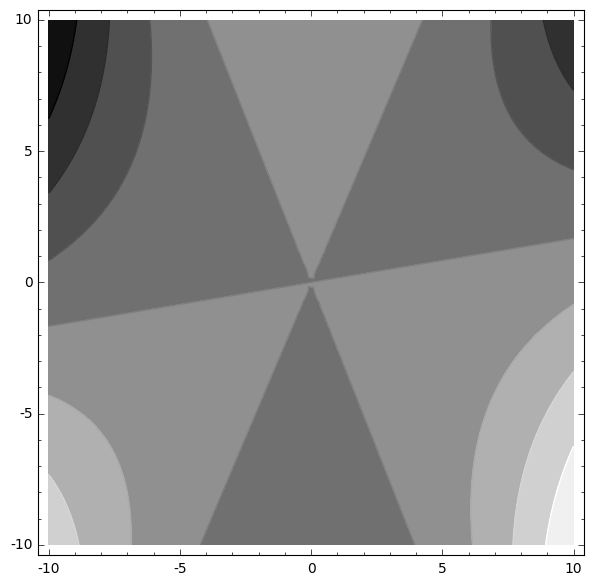
\includegraphics[width=5cm]{sage-algebraic-curve-plot}
\end{center}
from which we can see that our curve is a union of three lines.
Similarly
\begin{sageblock}
x,y=var('x,y')
contour_plot(y^2-x*(x-1)*(x-2)==0, (x,-3,4), (y,-5,5))
\end{sageblock}
yields level sets like
\begin{center}
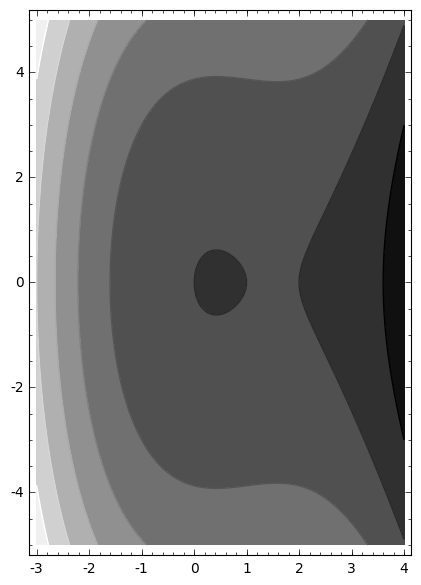
\includegraphics[width=5cm]{sage-algebraic-curve-plot-2}
\end{center}
and we can also plot the algebraic curve, without the other level sets, using
\begin{sageblock}
f(x,y) = y^2-x*(x-1)*(x-2)
implicit_plot(f, (-3, 4), (-5, 5))
\end{sageblock}
yielding
\begin{center}
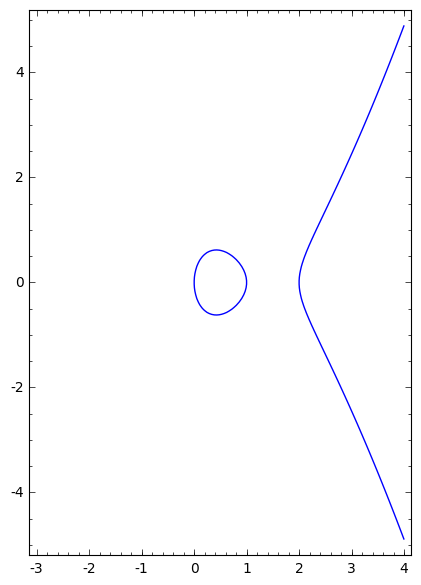
\includegraphics[width=5cm]{sage-algebraic-curve-plot-3}
\end{center}
Similarly, we can draw algebraic surfaces:
\begin{sageblock}
f(x,y,z) = y^2-x*(x-1)*(x-2)+z^4-1
implicit_plot3d(f, (-3, 4), (-5, 5), (-1,1))
\end{sageblock}
yielding
\begin{center}
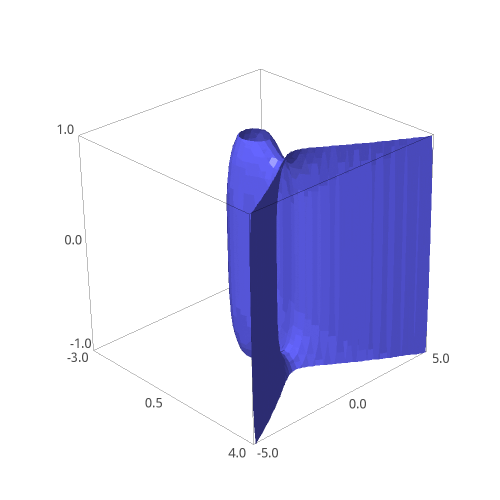
\includegraphics[width=5cm]{sage-algebraic-surface-plot}
\end{center}
